\documentclass[english]{article}

%These tell TeX which packages to use.
\usepackage{algorithm,algpseudocode}
\usepackage{array,epsfig}
\usepackage{amsmath}
\newcommand{\Mod}[1]{\ (\text{mod}\ #1)}
\usepackage{amsfonts}
\usepackage{amssymb}
\usepackage{amsxtra}
\usepackage{amsthm}
\usepackage{mathrsfs}
\usepackage{color}
\usepackage{listings}
\usepackage{matlab-prettifier}
\usepackage{multicol}
\usepackage{scrextend}
\usepackage{mathtools,calc}
\usepackage{caption}
\usepackage{subcaption}
\usepackage{float}
\usepackage{amssymb}
\usepackage{subcaption}
\usepackage{url}
\newcommand\hcancel[2][0.5pt]{%
  \ifmmode\sbox\CBox{$#2$}\else\sbox\CBox{#2}\fi%
  \makebox[0pt][l]{\usebox\CBox}%  
  \rule[0.5\ht\CBox-#1/2]{\wd\CBox}{#1}}
%\usepackage{kbordermatrix}


\usepackage{color} %red, green, blue, yellow, cyan, magenta, black, white
\definecolor{mygreen}{RGB}{28,172,0} % color values Red, Green, Blue
\definecolor{mylilas}{RGB}{170,55,241}


%Here I define some theorem styles and shortcut commands for symbols I use often
\theoremstyle{definition}
\newtheorem{defn}{Definition}
\newtheorem{thm}{Theorem}
\newtheorem{cor}{Corollary}
\newtheorem*{rmk}{Remark}
\newtheorem{lem}{Lemma}
\newtheorem*{joke}{Joke}
\newtheorem{ex}{Example}
\newtheorem*{soln}{Solution}
\newtheorem{prop}{Proposition}
\DeclareMathOperator*{\argmin}{arg\,min}
\DeclareMathOperator*{\argmax}{arg\,max}
\newcommand{\lra}{\longrightarrow}
\newcommand{\ra}{\rightarrow}
\newcommand{\surj}{\twoheadrightarrow}
\newcommand{\graph}{\mathrm{graph}}
\newcommand{\bb}[1]{\mathbb{#1}}
\newcommand{\Z}{\bb{Z}}
\newcommand{\Q}{\bb{Q}}
\newcommand{\R}{\bb{R}}
\newcommand{\C}{\bb{C}}
\newcommand{\N}{\bb{N}}
\newcommand{\M}{\mathbf{M}}
\newcommand{\m}{\mathbf{m}}
\newcommand{\MM}{\mathscr{M}}
\newcommand{\HH}{\mathscr{H}}
\newcommand{\Om}{\Omega}
\newcommand{\Ho}{\in\HH(\Om)}
\newcommand{\bd}{\partial}
\newcommand{\del}{\partial}
\newcommand{\bardel}{\overline\partial}
\newcommand{\textdf}[1]{\textbf{\textsf{#1}}\index{#1}}
\newcommand{\img}{\mathrm{img}}
\newcommand{\ip}[2]{\left\langle{#1},{#2}\right\rangle}
\newcommand{\inter}[1]{\mathrm{int}{#1}}
\newcommand{\exter}[1]{\mathrm{ext}{#1}}
\newcommand{\cl}[1]{\mathrm{cl}{#1}}
\newcommand{\ds}{\displaystyle}
\newcommand{\vol}{\mathrm{vol}}
\newcommand{\cnt}{\mathrm{ct}}
\newcommand{\osc}{\mathrm{osc}}
\newcommand{\LL}{\mathbf{L}}
\newcommand{\UU}{\mathbf{U}}
\newcommand{\support}{\mathrm{support}}
\newcommand{\AND}{\;\wedge\;}
\newcommand{\OR}{\;\vee\;}
\newcommand{\Oset}{\varnothing}
\newcommand{\st}{\ni}
\newcommand{\wh}{\widehat}
\newcommand\independent{\protect\mathpalette{\protect\independenT}{\perp}}
   \def\independenT#1#2{\mathrel{\rlap{$#1#2$}\mkern2mu{#1#2}}}

%Pagination stuff.
\setlength{\topmargin}{-.3 in}
\setlength{\oddsidemargin}{0in}
\setlength{\evensidemargin}{0in}
\setlength{\textheight}{9.in}
\setlength{\textwidth}{6.5in}

\newcommand{\pythonstyle}{\lstset{
language=Python,
keywordstyle=\color{blue},
stringstyle=\color{mylilas},
commentstyle=\color{mygreen},%
numbers=left,%
numberstyle={\tiny \color{black}},%
numbersep=9pt,
}}

\newcommand{\matlabstyle}{\lstset{language=Matlab,%
    %basicstyle=\color{red},
    breaklines=true,%
    morekeywords={matlab2tikz},
    keywordstyle=\color{blue},%
    morekeywords=[2]{1}, keywordstyle=[2]{\color{black}},
    identifierstyle=\color{black},%
    stringstyle=\color{mylilas},
    commentstyle=\color{mygreen},%
    showstringspaces=false,%without this there will be a symbol in the places where there is a space
    numbers=left,%
    numberstyle={\tiny \color{black}},% size of the numbers
    numbersep=9pt, % this defines how far the numbers are from the text
    emph=[1]{for,end,break},emphstyle=[1]\color{red}, %some words to emphasise
    %emph=[2]{word1,word2}, emphstyle=[2]{style},
}}

\begin{document}
\title{IRDM 2017 Project:\\Learning to Rank
}
\author{Group 42:\\
I-Horng Huang (12008651) \\
Tom Jakab\\
Phillip Mortimer (16052718)\\
\texttt{https://github.com/phillipmortimer/IRDM\_2017\_group\_42}}
\maketitle


\begin{abstract}
[TODO]
Required according to the problem sheet

\end{abstract}
\begin{multicols}{2}
\section{Introduction to the problem}
[TODO]


This project aims to explore the subject of Learning to rank. This is the problem of constructing a ranking model for information retrieval system, using machine learning techniques. 

Literature review of the subject is detailed in Section 2, with explanation of different approaches to Learning to Rank problem, including previous, and current state-of-the-art. Section 3 details the MSLR dataset used to perform experiments. 

Section 4 details the theory and results of the experiments, performed using different algorithms (RankNet, LambdaMART, MLP) under different metrics. Analysis of the results follows ..... 

[TODO]



\section{Literature review}

\subsection{Learning to rank}

Before machine learning techniques became popular, numerous algorithms were developed to rank documents by their relevance to a particular query.  These algorithms are now surpassed in performance by machine learning approaches, but they can still be used as features for machine learning algorithms. 

An important non-probabilistic ranking algorithms is the term frequency - inverse document frequency (TF-IDF) weighting \cite{tfidf}.  The TF measures the frequency of occurrence of a given term in a document.  The IDF weights terms which occur in a small number of documents in a collection more highly, as infrequently occurring are likely to be more discriminative.  In vector space ranking, the TF-IDF weighting is extended by representing the queries and documents as a TF-IDF vectors.   A ranking score is computed based on the cosine similarity between the TF-IDF vector of the query and the TF-IDF vector of documents in the corpus.  Probabilistic models estimate the probability that a user will find a given document relevant to a query.  The Okapi BM25 ranking is the considered the benchmark model of this type.  It is derived from modelling the distribution of within-document frequencies of a relevant
term as a mixture of two Poisson distributions \cite{robertson1993okapi}.

These approaches are all essentially hand-designed algorithms which use only a small number of features.  Given training data of queries $q$, documents $d$ and a relevance or rank score $y$, we can \textit{learn} to predict $y$ for a new query-document pair.  Machine learning techniques to do this are generally categorized into three approaches: \textit{pointwise}, \textit{pairwise} and \textit{listwise}.  We review these approaches in the following sections.

\subsection{Pointwise methods}

In pointwise approaches the training data consists of triples $(\mathbf{q}, \mathbf{d}, y)$.  We train a ranking rule $h(\mathbf{w}, \phi (\mathbf{q}, \mathbf{d})) = y$, where $\phi$ is a mapping from query-document pairs to features and $\mathbf{w}$ is a vector of parameter weights.  Depending on how relevance is measured, this can be posed as a regression, classification or ordinal regression problem.  

PRank \cite{crammer2001pranking} (Perceptron Ranking) is an online ranking algorithm with an update rule motivated by the classic perceptron algorithm.  The relevance rank is considered to be an ordered set $\{1, 2, \ldots, k \}$.  The ranking rule maintains a vector $\mathbf{w}$ and a series of thresholds $b_1 \le b_2 \ldots b_{k-1} \le b_k = \infty$.  Given a new instance $x$, the predicted rank is defined to be the index of the first threshold $b_r$ for which $\mathbf{w}^T \mathbf{x} < b_r$.  During training an instance $\mathbf{x}_t$ is received and the estimated rank $\hat{y}_t$ is calculated.  If $\hat{y}_t \ne y_t$, then $\mathbf{w}$ and the thresholds $b_r$ are updated according to a perceptron-like algorithm.  

Pointwise approaches are widely used because of their simplicity and effectiveness.  However, a problem with pointwise methods is that the loss function used in training the model will be dominated by those queries which match a large number of documents.  The loss function also does not take into account the position of documents in the ranking list, which can lead to unimportant documents being given too much weight.

\subsection{Pairwise methods}

Tom to complete

\subsection{Listwise methods}

One problem with pairwise approach is that the loss function is suboptimal, in the sense that it is not optimizing for the evaluation methods directly. Another problem is that position in ranking and number of documents per query are not taken into account. Listwise approaches to learning to rank problem tries to optimize directly for the chosen evaluation metrics. However, this is difficult as cost functions are often non-continuous. Approximations or bounds can be taken to simplify this problem.

One probabilistic model for ranking is the ListNet \cite{cao2007learning}. Suppose that there is a ranking function which assigns scores to $n$ objects. A ranked list scores are mapped to a probabilistic distribution, such as Permutation probability:
$$P_s(\pi) = \prod_{j=1}^n \frac{\phi(s_{\pi(j)})}{\sum^n_{k=j} \phi(s_{\pi(k)})} $$
where $s_{\pi(j)}$ denotes score of object at position j of permutation $\pi$, such as the exponential function. The loss function is then the KL-divergence between Top-k distributions. This can be modeled using neural networks and optimized using various gradient descent algorithm.

Another listwise approach is Adarank \cite{xu2007adarank}. Inspired by the Adaboost algorithm [citation], Adarank uses a linear combination of weak ranker $h_t$ to form a strong ranker: $f(x) = \sum^T_{t=1} \alpha_t h_t(x)$. The algorithm takes in a training set, initially, it sets all weights $\alpha_t$ to be equal, and iteratively increase the weightings of weak learners that perform badly, in order to work on harder queries in the next iteration. 

\subsection{Deep learning in ranking systems}

We survey some recent papers in this field and summarize their findings.

Deep convolutional networks have recently been applied to ranking text pairs by Severyn and Moschetti \cite{severyn2015learning}.  Their approach combines a simple pointwise ranking with a deep learning architecture to create a rich representation of query-document pairs.  First, a \textit{sentence model} uses a deep convolutional network to map queries or documents to an intermediate representation.  Second, a \textit{matching model} receives (query representation)-(document representation) pairs form the sentence model and learns the semantic matching between the corresponding input query-document pairs.  The matching model is also a  deep convolutional network.  The model was trained and tested on TREC microblogging datasets from 2011 and 2012, consisting of 16M tweets.  It achieved mean average precision performance on par with previous state-of-the-art, even though the model requires no manual feature engineering and minimal pre-processing.

Another recent approach to this is to use attention based methods applying to  learning to rank problem \cite{wang2017attention} in a listwise fashion. The contribution of the paper is that it takes different embeddings of queries (such as TF-IDF, LSA, word2vec) into account, and incorporating them with the attention mechanism. Additionally, attention mechanism is also applied to the search results. This is done by attaching the attention layer on top of both queries and ranks, the output of each attention layer is feed into each of the two layer recurrent neural network, and then output a softmax score that are used as ranking prediction. The model can be train end-to-end using popular optimization approaches. This model was applied to the 20 Newsgroups data set with 18k documents and 7 superclasses and achieve state-of-the-art performance across $MAP, NDCG_3$ and $NDCG_5$ error metrics. Additionally, this model can also be applied to image queries, where one can add Convolutional layers that feeds  into the embedding layer as image features. The result of this is shown in the paper with MNIST and CIFAR-10 dataset.

\section{Dataset}

The MSLR dataset \cite{DBLP:journals/corr/QinL13} was released by Microsoft Research in 2010.  The dataset is available in two size: MSLR-WEB30k with more than 30,000 queries and a random sampling from it, MSLR-WEB10k.  Here we use the smaller MSLR-WEB10k dataset.  The data is in the form of url-query pairs, with a relevance score obtained from the Microsoft Bing search engine, ranging from 0 (irrelevant) to 4 (perfectly relevant).  Features have been pre-extracted as a 136 element vector, comprising numerous standard features used in information retrieval, such term frequency, TF-IDF, BM25 and URL properties.

The full dataset is partitioned into 5 subsets and these are presented as 5 folds, where each fold consists of three of the five partitions for training, one for validation and one for testing.  

\subsection{Dataset statistics}

The dataset contains 1.2 million document-query pairs.  There are 10,000 queries, giving an average number of documents per query of 120.

\section{Experiments}

\subsection{RankNet}

RankNet takes input feature vector $x$ and mapped it into a score $s$. It compares the scores of two urls using a sigmoid function and compute a loss function (for instance, using cross entropy). The algorithm can then optimize the neural network using the aggregated loss.

The RankLib \cite{Lemur} implementation of RankNet was used.  Parameter tuning was performed for the learning rate, number of layers and number of nodes.  The learning rate $\alpha$ was varied in the range $\alpha \in \{10^{-2},10^{-3} \ldots, 10^{-6}\}$, the number of nodes in the hidden layer varied in the range $\{5, 10, 20\}$ and the number of layers in $\{1, 2\}$.  Training was continued over 20 epochs of the dataset and was run in parallel for each combination of layers and nodes using multiple AWS instances.  Performance on the held out test set was evaluated using nDCG@10. 

Input features were normalized to lie in the range $[-1,1]$ before being fed to RankNet.  This is achieved using the linear normalization option of the RankLib library.  Feature normalization is import for neural networks to ensure that initial activations lie close to the linear region of the activation function.  Without this, gradients cannot back-propagate and training of the network is difficult. 

The best nDCG@10 during training is shown in Table \ref{tab:RankNet_train}.  The single layer network with 20 nodes offered the best performance.  Training was also completed with 40 nodes using the best learning rate from the 20 node model, but it gave almost no improvement in performance, but was significantly slower to train. 

\begin{table}[H]
\begin{center}
\begin{tabular}{c c c c c c}
  \hline
  {} & {} & \multicolumn{4}{c}{Number of nodes}\\
  $\alpha$ & Layers & 5 & 10 & 20 & 40\\
  \hline
  $10^{-2}$ & 1 & 0.1833 & 0.1837 & 0.1862 & - \\
  $10^{-3}$ & 1 & 0.1866 & 0.1839 & 0.1838 & - \\
  $10^{-4}$ & 1 & 0.1958 & 0.2089 & 0.3527 & - \\
  $10^{-5}$ & 1 & 0.3107 & 0.3193 & 0.3671 & 0.3676\\
  $10^{-6}$ & 1 & 0.3039 & 0.3077 & 0.3199 & - \\
  \hline
  $10^{-2}$ & 2 & 0.1856 & 0.1861 & 0.1832 & - \\
  $10^{-3}$ & 2 & 0.1869 & 0.1866 & 0.1861 & - \\
  $10^{-4}$ & 2 & 0.3166 & 0.3082 & 0.3370 & - \\
  $10^{-5}$ & 2 & 0.3103 & 0.3159 & 0.3130 & - \\
  $10^{-6}$ & 2 & 0.2783 & 0.3089 & 0.2960 & - \\
  \hline
\end{tabular}
\caption{\label{tab:RankNet_train}RankNet best test nDCG@10 for different learning rates $\alpha$ and network architectures.}
\end{center}
\end{table}

Note that the best performance was not necessarily seen at the end of the training over 20 epochs.  This can clearly be seen from the learning curves shown in Figures \ref{fig:RankNet_1_lc} and \ref{fig:RankNet_2_lc}.  Performance initially rises, before falling as the network starts to over-fit the training data.  The final ranking algorithm was then trained using early stopping, to prevent over-fitting.  

\begin{figure}[H]
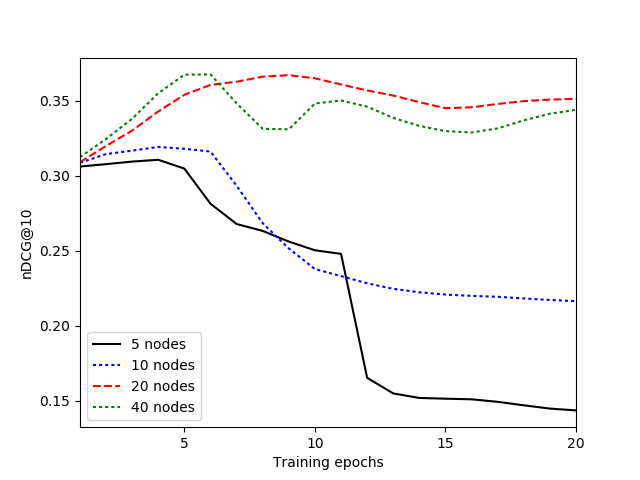
\includegraphics[width=\linewidth]{figures/RankNet_1_layer_training.png}
\caption{RankLib learning curves for $\alpha=10^{-5}$: single layer network.  The reported nDCG@10 is on the training data.} \label{fig:RankNet_1_lc}
\end{figure}

\begin{figure}[H]
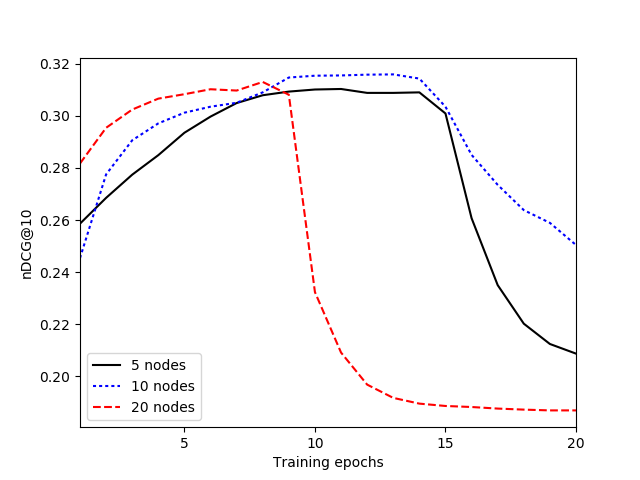
\includegraphics[width=\linewidth]{figures/RankNet_2_layer_training.png}
\caption{RankLib learning curves for $\alpha=10^{-5}$: two layer network.  The reported nDCG@10 is on the training data.} \label{fig:RankNet_2_lc}
\label{RankLib_lc}
\end{figure}

\subsection{LambdaMART}

RankNet approaches are optimized for the pairwise error, but this might not match well with other information retrieval measures. The idea of LambdaRank is to write down the desired gradient directly, if $U_1$ is more relevant than $U_2$, increase the rank of the former by $|\lambda|$ and decrease the latter by the same amount. $\lambda$ can be written down based on the evaluation measures \cite{burges2010ranknet}. 
LambdaMART is a combination of LambdaRank and MART (Multiple Additive Regression Trees) \cite{mart}. LambdaMART uses gradient boosted decision trees using a cost function derived from LambdaRank to solve the learning to rank problem.


RankLib \cite{Lemur} implementation of LambdaMART was used to perform the experiments. Combinations of parameters are run: number of leaf $\{1,10,100,1000\}$, learning rate (shrinkage) $\{10^{-2}, 10^{-1}, 10^{0}\}$ and threshold candidate $\{64,256\}$. All experiments are run over 250 iterations (number of trees) with minimum leaf support = 1, evaluate with nDCG@10.

The best nDCG@10 on test set is shown in Table \ref{tab:LambdaMART_train}. The best nDCG@10 performing architecture during training is with $\alpha = 10^{-1}, tc = 256,$ number of leaf $= 1000$. Figure \ref{fig:LambdaMART_lc} shows the general trends of how each parameters effects learning curve: the higher number of leaf tends to have positive impacts on nDCG@10, and threshold candidates number have no significant impact on training performance. Both diagram and table also shows that beyond around 0.45 nDCG@10, the learning procedure starts to overfits. 

\begin{table}[H]
\begin{center}
\begin{tabular}{c c c c c c}
  \hline
  {} & {} & \multicolumn{4}{c}{Number of Leaves}\\
  $\alpha$ & tc & 1 & 10 & 100 & 1000\\
  \hline
  $10^{-2}$ & 64 & 0.3041 & 0.4021 & 0.4182 & 0.4250 \\
  $10^{-1}$ & 64 & 0.4068 & 0.4423 & 0.4481 & 0.4441 \\
  $10^{0}$ & 64 & 0.3371 & 0.4236 & - & - \\
  \hline
  $10^{-2}$ & 256 & 0.3001 & 0.3993 & 0.4185 & 0.4261 \\
  $10^{-1}$ & 256 & 0.4074 & 0.4407 & 0.4501 & - \\
  $10^{0}$ & 256 & 0.3335 & 0.4255 & - & - \\
  \hline
\end{tabular}
\caption{\label{tab:LambdaMART_train}LambdaMART best test nDCG@10 for different learning rates (shrinkage) $\alpha$ and parameter combinations.}
\end{center}
\end{table}

\begin{figure}[H]
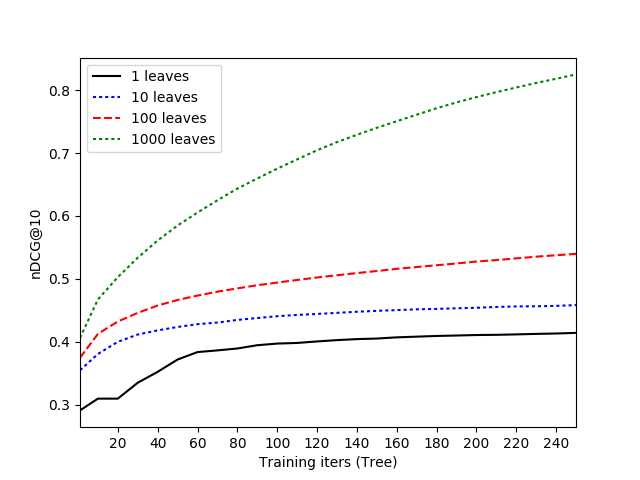
\includegraphics[width=\linewidth]{figures/LambdaMART_64_training.png}
\caption{LambdaMart learning curves (training nDCG@10) for $\alpha=10^{-1}$, tc = 64 for 250 iterations } \label{fig:LambdaMART_lc}
\label{LambdaMART_lc}
\end{figure}

\subsection{AdaRank}

AdaRank is a boosting algorithm, that minimizes a loss function directly related to performance measures such as nDCG \cite{Xu2007AdaRankAB}.  We again use the RankLib implementation of this algorithm.  

We tune the tolerance parameter in the range $\{0.01, 0.002, 0.005, 0.001, 0.0005\}$.  This parameter determines whether to continue with another round of training if the improvement between rounds is less than the tolerance.  We tune the paramater \emph{max} in the range $\{1, 2, 5, 10, 20\}$.  This parameter controls the maximum number of times can a feature be consecutively selected without changing performance.
Results are shown in Table \ref{tab:AdaRank_train}.

\begin{table}[H]
\begin{center}
\begin{tabular}{c c c c}
  \hline
  Max rounds & Tolerance & Max & nDCG@10\\
  \hline
  500 & 0.01 & 5 & 0.2808 \\
  500 & 0.005 & 5 & 0.2808 \\
  500 & 0.002 & 5 & 0.3976 \\
  500 & 0.001 & 5 & 0.3976 \\
  500 & 0.0005 & 5 & 0.3976 \\
  \hline
  500 & 0.002 & 1 & 0.3976 \\
  500 & 0.002 & 2 & 0.3976 \\
  500 & 0.002 & 5 & 0.3976 \\
  500 & 0.002 & 10 & 0.3976 \\
  500 & 0.002 & 20 & 0.3976 \\
  \hline
\end{tabular}
\caption{\label{tab:AdaRank_train}AdaRank best test nDCG@10 for parameter combinations.  The feature max refers to the maximum number of times can a feature be consecutively selected without changing performance.}
\end{center}
\end{table}

\subsection{Logistic regression classifier}

logistic regression

\subsection{Multi-layer perceptron}

MLP

\subsection{Metrics and Results}

\section{Analysis of results}

\subsection{Effect of parameter tuning on performance}

Effect of parameter tuning on performance.  

\subsection{Comparison of ranking algorithms}

Comparison

\section{Discussion and limitations}

\section{Conclusion}

\newpage
\medskip

\bibliographystyle{unsrt}
\bibliography{IRDM_42}
\end{multicols}
\end{document}